\section{Mechanical Design}

\subsection{Screw Feeder}
% TODO: FIX Citation and Picture
\begin{figure}[h]
\centering
\includegraphics[width=6cm]{screw feeder} % replace with image path
\caption{Screw Feeder Diagram}
\label{fig:screw_feeder}
\end{figure}

% TODO: Update Citation
Figure\ref{fig:screw_feeder} shows the diagram of a screw feeder. Screw feeders are usually used in industrial fields like agriculture, chemicals, plastics, cements, poultry and food processing. According to Mingalani et al. (2020), screw feeders are specifically used to transport or move granular materials at a controlled rate like corn and wheat. It consists of a rotating screw and small feeding section or the hopper. Despite having big batches of a certain material, screw feeders can control the rate of which these materials are dispensed. With this concept, the group decided to utilize a screw feeder as the input mechanism for the system. This mechanism allows a controlled rate of coffee bean dispensing, which is a significant factor to avoid overcrowding in the rotating conveyor table causing the beans to jam. In addition, batches of coffee beans can be put at once instead of just adding a certain amount of beans at a time. 

\subsection{Rotating Conveyor Table}
\begin{figure}[h]
    \centering
    \includegraphics[width=6cm]{rotating conveyor table} % replace with image path
    \caption{Rotating Conveyor Table 3D Design (32-inch Rotary Table Accumulator (RTA))}
    \label{fig:rotating_conveyor_table}
\end{figure}

After the inputted beans comes out from the screw feeder, the coffee beans would then be placed in the rotating conveyor table. According to the study of Dabek (2022). The conveyor table is used as a transportation systems for all forms of bulk materials to a certain machine or destination. The system utilizes the rotating conveyor table to have a controlled movement of coffee beans towards the first stage of the system. The improvised linearization system, consisting of metal guide rails and dividers ensures that beans align in a single path, reducing random movement, and improving the flow of the input beans. An infrared sensor would detect each bean as it passes, to control the movement of the bean preventing clogging and ensuring efficient operation. 

\subsection{Inspection Tray (1st Stage)}

\begin{figure}[h]
    \centering
    \includegraphics[width=6cm]{inspection tray design} % replace with image path
    \caption{Inspector Tray 3D Design}
    \label{fig:inspection_tray}
\end{figure}

The inspection tray serves as the platform for the machine vision based analysis of coffee beans. It is designed with 8 holes, allowing uniform placements and optimal camera positioning for the system. The system utilizes a two-layer structure: a stationary acrylic platform and a rotating 3D-printed platform with holes. The rotating mechanism sequentially positions each bean between two webcams, which captures and analyzes its physical characteristics from top and bottom perspective. This design captures both sides of the bean, ensuring a better classification of the bean. After inspection, the bean moves onto a slide, where it is either directed to the second stage for density analysis (Good) or sorted out as a defect.

\subsection{Density Sorter (2nd Stage)}
% ! MISSING CONTENT

\section{Embedded Systems}

\subsection{Microcontroller}

\begin{figure}[h]
    \centering
    \includegraphics[width=6cm]{arduino nano} % replace with image path
    \caption{Arduino Nano Microcontroller}
    \label{fig:arduino_nano}
\end{figure}

Since the system is composed of two stages of sorting: defect sorting through computer vision and density-based analysis–the group decided to utilize two Arduino Nano microcontrollers to modularize the control process. The first Arduino Nano microcontroller is tasked to handle the computer vision-based defect sorting through serial communication with OpenCv operating in Python. In addition, it handles the operation of defect sorting consisting of a stepper motor for the rotation of the inspection tray and a servo motor for the slider, which directs the beans to the designated bin (defect or good bin). On the other hand, the second Arduino Nano microcontroller manages the density-based analysis and sorting, which consists of another stepper motor to direct the beans to its respective bin (dense and less-dense bin), the precision scale which is interfaced through RS232, and the top feeder where the input beans are poured. The use of separate Arduino microcontrollers is advantageous when it comes to the computer vision-based sorting of beans. This is because serial communication is much faster when code complexity is significantly reduced. With this, a designated microcontroller handles the computer vision part and two-way serial communication between the microcontroller and the computer vision algorithm running in Python. Most importantly, the use of two microcontrollers allowed the system to not rely solely on a sequential approach. This means that the two stages of sorting are not relying on the timing of each other, allowing the inspection tray and the top feeder to operate independently. Thus, resulting in a much faster and efficient sorting process. 

\subsection{Sensors}

\begin{figure}[h]
    \centering
    \includegraphics[width=6cm]{infrared sensor} % replace with image path
    \caption{Infrared Sensor}
    \label{fig:infrared_sensor}
\end{figure}

To ensure that the beans are falling in a one-by-one manner onto the inspection tray, the group placed an IR sensor at the edge of the top feeder. This IR sensor triggers the DC motor that runs the feeder to stop, and runs small steps until the bean is dropped. The addition of the IR sensor at the edge of the feeder allows the motor to run continuously until another bean is detected. With this, the waiting time for the next bean at the inspection tray is significantly lessened. 

\begin{figure}[h]
    \centering
    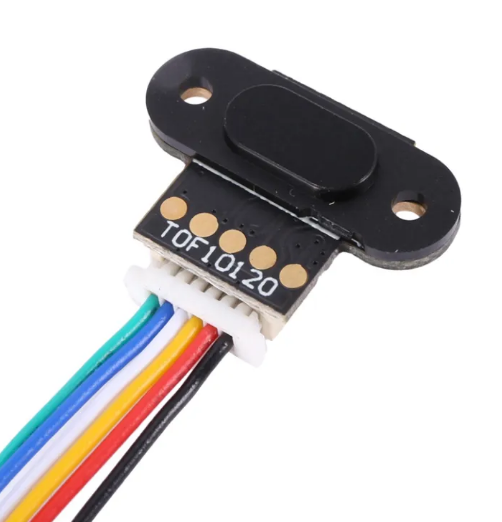
\includegraphics[width=6cm]{TOF10120} % replace with image path
    \caption{TOF10120}
    \label{fig:tof10120}
\end{figure}

TOF10120 or Time of Flight sensor is utilized in the system due to its high precision, non-contact measurement capability. This sensor is used to estimate the volume of each bean, which is essential for computing the density. In the second stage of sorting, where beans are classified based on density, the sensor plays a crucial role in determining the approximate volume of each bean by measuring its height or dimensions as it passes through the system.

\subsection{Motor control}

\begin{figure}[h]
    \centering
    \includegraphics[width=6cm]{stepper_motor} % replace with image path
    \caption{12V NEMA 17 Stepper Motor}
    \label{fig:stepper_motor}
\end{figure}

Two NEMA 17 12V stepper motors, paired with L298N motor drivers were used to control the movement of the inspection tray in the first stage and the density-based sorting mechanisms in the second stage. In these mechanisms, the group decided to use stepper motors to ensure precise and accurate movements. Precise and accurate movements are needed for the inspection tray to make sure every movement of the hole is perfectly aligned to the camera. Thus, allowing a more uniform and consistent angle for each bean to be inspected through the computer vision. In addition, NEMA 17 stepper motors were the best choice for these mechanisms due to its high torque, which is essential because it will be moving weighted objects. 

\begin{figure}[h]
    \centering
    \includegraphics[width=6cm]{6v_dc_motor} % replace with image path
    \caption{6V DC Motor}
    \label{fig:6v_dc_motor}
\end{figure}

For the rotating conveyor table (top feeder), where the beans are initially poured, a 6V DC motor is used. The group decided to use this motor due to its high RPM, which is needed for a fast rotation of the rotating conveyor table. The speed of the feeder is regulated to prevent clogging and ensure that the beans are evenly spaced before they enter the inspection tray. The motor speed is fine-tuned through pulse-width modulation (PWM) to synchronize with the stepper motor-driven inspection tray, ensuring a steady input without overwhelming the system.

\begin{figure}[h]
    \centering
    \includegraphics[width=6cm]{motor driver} % replace with image path
    \caption{TB6612FNG Motor Driver}
    \label{fig:motor_driver}
\end{figure}

To drive the 6V DC motor, the group utilized TB6612FNG, a motor driver module. This module also allowed PWM control for the motor, which is essential for reducing the speed of the motor when needed. 

\subsection{Operating Voltage}

\begin{figure}[h]
    \centering
    \includegraphics[width=6cm]{12v power supply} % replace with image path
    \caption{12V Power Supply}
    \label{fig:12v_power_supply}
\end{figure}

The main power supply comes from a 12V external power supply, which provides enough voltage for all the components and keeps the voltage from dropping and interfering with system performance. The Arduino microcontroller is powered via its VIN pin, so it can function without the need for a USB connection and maintains a stable 5V logic output for sensor and actuator control. The NEMA 17 stepper motors that operate the inspection tray and density sorter are directly powered from the 12V supply and fed into L298N motor drivers to adjust voltage and monitor current flow. Operating these motors at 12V provides best torque output, which is vital in ensuring consistent movement during the sorting process.

\begin{figure}[h]
    \centering
    \includegraphics[width=6cm]{stepup module} % replace with image path
    \caption{MT3608 Step-Up Module}
    \label{fig:mt3608}
\end{figure}

For the top feeder mechanism, a step-up module is needed to supply the sufficient voltage needed for the motor–6V. From the 5V output of the Arduino, the step-up module will be utilized to convert it into 6V.

\section{Computer Vision System}
% TODO: Write content
\subsection{Image Processing}
\subsection{Image Detection and Classification Models}

\section{Serial Communication}

Serial communication is used for sensors and motors for arduino due to the simplicity, reliability and efficient transfer of data between different devices. The precision scale uses a RS232 and a MAX TTL converter to send the data from the precision to the arduino to get the weight values of each green coffee bean. To sort out the good from defective beans the system utilizes a servo motor. The data from python is received by the arduino through serial communication. The python side is responsible for the decision and defect classification while the arduino is responsible for controlling the servo motor.  

\section{Graphical User Interface (GUI)}

% TODO: Update design to consider new features (Tracking which defects are present, the recommendation based on thresholding, the speed of system, runtime ,etc.)
\begin{figure}[h]
    \centering
    \includegraphics[width=6cm]{gui} % replace with image path
    \caption{Graphical User Interface}
    \label{fig:gui}
\end{figure}

The proposed system would be integrating a graphical user interface developed using PyGui and ChatGPT API. The GUI would serve as the control center platform for the system. This would provide real-time feedback and insights for users. As shown in Figure 8, a concept of how the GUI would interact with the system would be a start button, once the button is executed the system would then be expecting inputs and start sorting. There would be real-time feedback during the sorting process, then some visual markers to indicate their classification, and an elapsed time so the user would be aware of the time of the sorting process. Once the system is done, the user can click the end button and the summary report would generate in an orderly manner, providing tables of classification that was detected through the process. In the bottom part of the GUI, ChatGPT API would be integrated and would offer recommendations based on the detected quality and classification of the coffee beans. 

\section{Density Based Analysis}
% TODO: Write contentmt3608

\section{Summary}
\lipsum